\documentclass[12pt,article]{article}
\usepackage{lmodern}
\usepackage{amssymb,amsmath}
\usepackage{ifxetex,ifluatex}
\usepackage{fixltx2e} % provides \textsubscript
\ifnum 0\ifxetex 1\fi\ifluatex 1\fi=0 % if pdftex
  \usepackage[T1]{fontenc}
  \usepackage[utf8]{inputenc}
\else % if luatex or xelatex
  \ifxetex
    \usepackage{mathspec}
    \usepackage{xltxtra,xunicode}
  \else
    \usepackage{fontspec}
  \fi
  \defaultfontfeatures{Mapping=tex-text,Scale=MatchLowercase}
  \newcommand{\euro}{€}
\fi
% use upquote if available, for straight quotes in verbatim environments
\IfFileExists{upquote.sty}{\usepackage{upquote}}{}
% use microtype if available
\IfFileExists{microtype.sty}{%
\usepackage{microtype}
\UseMicrotypeSet[protrusion]{basicmath} % disable protrusion for tt fonts
}{}
\usepackage[margin=1.25in]{geometry}
\usepackage{graphicx}
\makeatletter
\def\maxwidth{\ifdim\Gin@nat@width>\linewidth\linewidth\else\Gin@nat@width\fi}
\def\maxheight{\ifdim\Gin@nat@height>\textheight\textheight\else\Gin@nat@height\fi}
\makeatother
% Scale images if necessary, so that they will not overflow the page
% margins by default, and it is still possible to overwrite the defaults
% using explicit options in \includegraphics[width, height, ...]{}
\setkeys{Gin}{width=\maxwidth,height=\maxheight,keepaspectratio}
\ifxetex
  \usepackage[setpagesize=false, % page size defined by xetex
              unicode=false, % unicode breaks when used with xetex
              xetex]{hyperref}
\else
  \usepackage[unicode=true]{hyperref}
\fi
\hypersetup{breaklinks=true,
            bookmarks=true,
            pdfauthor={},
            pdftitle={Does Public Support for UKIP Drive Media Coverage or Does Media Coverage Drive Support for UKIP?},
            colorlinks=true,
            citecolor=blue,
            urlcolor=blue,
            linkcolor=blue,
            pdfborder={0 0 0}}
\urlstyle{same}  % don't use monospace font for urls
\setlength{\parindent}{0pt}
\setlength{\parskip}{6pt plus 2pt minus 1pt}
\setlength{\emergencystretch}{3em}  % prevent overfull lines
\setcounter{secnumdepth}{0}

%%% Use protect on footnotes to avoid problems with footnotes in titles
\let\rmarkdownfootnote\footnote%
\def\footnote{\protect\rmarkdownfootnote}

%%% Change title format to be more compact
\usepackage{titling}
\setlength{\droptitle}{-2em}
  \title{Does Public Support for UKIP Drive Media Coverage or Does Media Coverage
Drive Support for UKIP?}
  \pretitle{\vspace{\droptitle}\centering\huge}
  \posttitle{\par}
  \author{Justin Murphy\\University of Southampton}
  \preauthor{\centering\large\emph}
  \postauthor{\par}
  \date{}
  \predate{}\postdate{}


\usepackage{dcolumn}
\usepackage{setspace}


\begin{document}

\maketitle


This research note presents the first statistical time-series analysis
testing the degree to which media coverage of UKIP is driven by public
support for UKIP and/or vice versa. In particular, I gather monthly
time-series of public support for UKIP from Ipsos MORI's voting
intention polls and a monthly count of UKIP mentions in all UK National
Newspapers (drawn from the databse Nexis). I begin with a series of
econometric analyses to investigate whether media coverage drives
support, support drives media coverage, or both. First,
vector-autoregression (VAR) is used as a straightforward and relatively
atheoretical way to document the stylized facts of the causal dynamics.
Then, separate error-correction models are estimated as an alternative
approach to the question making different assumptions. Finally, I
provide a brief qualitative examination of the time-series. Both
econometric techniques and the qualitative evidence converge on the
conclusion that the relationship between public support and media
coverage of UKIP is one of positive feedback: while public support is
positively correlated with future levels of media coverage, media
coverage is also independently correlated with future increases in
public support. Qualitative exploration of these dynamics identify at
least two key time periods in which support for UKIP was decreasing but
media coverage increased and may have caused support for UKIP to
increase: a surge in media coverage in the second half of 2012, not
triggered by any public support, was followed by a surge of support
which came in the first half of 2013. Then, despite \emph{decreasing}
support throughout 2013, media coverage increases briefly before surging
in the second half of 2013 until the middle of 2014, apparently helping
to maintain current levels of support.

\pagebreak

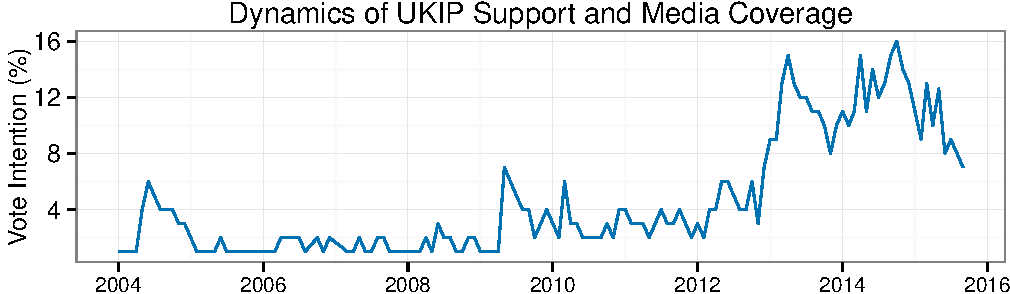
\includegraphics{ukip_media_files/figure-latex/unnamed-chunk-11.pdf}
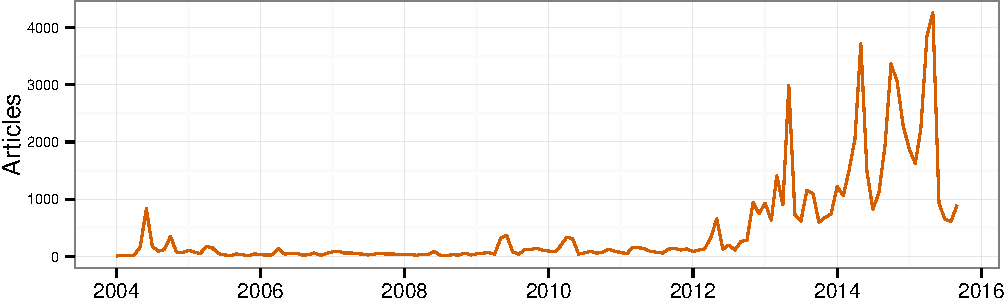
\includegraphics{ukip_media_files/figure-latex/unnamed-chunk-12.pdf}

\begin{figure}[htbp]
\centering
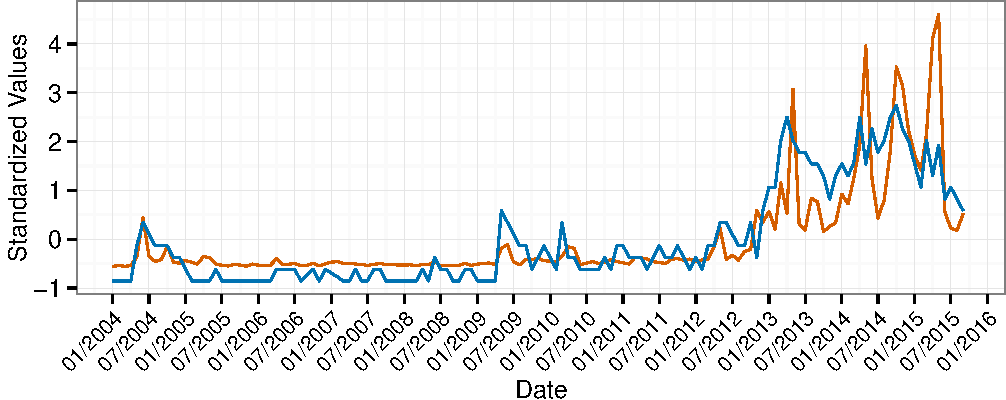
\includegraphics{ukip_media_files/figure-latex/unnamed-chunk-2.pdf}
\caption{Dynamics of UKIP Support and Media Coverage}
\end{figure}

\section{Background and Literature
Review}\label{background-and-literature-review}

Critics allege that the media pays disproportionate attention to UKIP
but media elites claim that coverage of UKIP is driven by increasing
public support for the party. It is widely argued in the popular press,
by scholars as well as politicians, that the British media pays
disproportionate attention to UKIP (Goodwin and Ford 2013; Stevenson
2014; Soussi 2014). This is uncontroversial in the sense that the
quantity of UKIP's media coverage is simply much greater than the
coverage of other small parties on the right as well as the left
(Goodwin and Ford 2013). Statements by UK media regulator Ofcom as well
as the BBC suggest that UKIP deserves more coverage than other
relatively small parties because of uniquely growing public support for
UKIP (Sweeney 2015; Wintour 2015).

The crucial and controversial question--and the motivation for this
article--is whether the quantity of UKIP's media coverage represents a
form of media bias with negative implications for democracy, or if the
media's fascination with UKIP is merely a reasonable or even healthy
response to a newly rising political party. If disproportionate media
coverage is not simply responsive to public opinion but effectively
driving public opinion and shaping outcomes such as elections, as some
argue (Soussi 2014), then clearly the media's disproportionate coverage
of UKIP is at best normatively problematic and at worst complicit in the
legitimation and empowerment of what is alleged to be UKIP's coded
racism and proto-fascism (Webb 2014; Syal 2015).

While a great deal of research documents various aspects of the
relationship between media and right-wing populist parties, little is
known specifically about the effects of the quantity of party-specific
media coverage on aggregate party support from a dynamic perspective.
The closest previous research comes to this particular question is work
by (Boomgaarden and Vliegenthart 2007; Boomgaarden and Vliegenthart
2009), who find that greater media coverage of immigration issues is
positively associated with support for anti-immigration parties. Other
research has studied the dynamics of individual-level exposure to media
coverage and perceptions of right-wing politicians (Bos, Brug, and
Vreese 2011). Still, currently extant research tells us surprisingly
little about the causal dynamics of public support and the quanitity of
media coverage of right-wing populist parties. In part, this may be
because the application of time-series techniques to aggregate media
data remains relatively under-explored (Vliegenthart 2014).

\section{Hypotheses}\label{hypotheses}

Hypothesis 1: Public support for UKIP and media coverage of UKIP are
characterized by positive feedback, wherein an increase in either
variable leads to an increase in the other variable.

\begin{itemize}
\item
  Hypothesis 1.A: Increases in public support for UKIP lead to increased
  media coverage, controlling for previous levels of media coverage.
\item
  Hypothesis 1.B: Increases in media coverage lead to increased public
  support, controlling for previous levels of public support.
\end{itemize}

Hypothesis 3: Exogenous increases in media coverage (not preceded by
increases in public support) have led to increases in public support.

\section{Data, Method, and Research
Strategy}\label{data-method-and-research-strategy}

To measure public support for UKIP, I gathered monthly aggregate polling
data on vote intentions from Ipsos MORI (Ipsos-MORI). Specifically, I
constructed a variable from the percentage reporting an intention to
vote for UKIP according to the Ipsos MORI poll closest to the middle of
each month. For most months, this was straightforward because the Ipsos
MORI poll is approximately monthly. For months with multiple polls, I
used the poll closest to the middle of the month. For the very few
months with no poll or a poll at the border between the previous or
following month, the value was counted as missing and then all missing
values were linearly interpolated. To measure media coverage of UKIP, I
gathered monthly counts of all UK national newspaper reports mentioning
either ``UKIP'' or ``UK Independence Party'' from the database Nexis
(``Nexis'').\footnote{Duplicate articles defined by Nexis's definition of high similarity were excluded.}

Econometric techniques are used to test for, and distinguish the
ordering of, potential causal dynamics between media coverage and public
support for UKIP. A brief qualitative historical analysis of these
dynamics will be used to better understand a potential causal process.
In particular, the substantive nature of the puzzle at hand requires the
identification of a causal narrative. Even with econometric evidence
suggesting an independent causal effect from either one to the other, it
would not be clear whether the historical unfolding of these causal
dynamics implies a problem for democracy. We are not only interested in
whether media coverage amplifies exogenous increases in support--this
would be an important but not necessarily problematic finding from a
democratic perspective--but whether increases in media coverage have
generated support for UKIP despite low, stagnant, or decreasing levels
of support.

\section{Analysis}\label{analysis}

\subsection{VAR}\label{var}

Because both variables are non-stationary, vector autoregression is
estimated with first differences of each variable. Optimal lag length is
determined by the Aikeke Information Criterion to be to be VAR(3). The
model includes a constant and a trend term. Diagnostics suggest that
using the log of each variable before differencing reduces
heteroskedasticity and serial correlation of errors. Because VAR models
have many paramaters to begin with, monthly indicators controlling for
seasonality absorb crucial degrees of freedom and so are excluded in the
intitial models but added in subsequent models. The models displayed
here all pass the standard ARCH-LM and Portmanteau tests for
non-constant error variance and serial correlation of errors,
respectively. Finally, diagnostics show no evidence of significant
temporal instability (see Supplementary Information).

Surprisingly, initial VAR results show little evidence that changes in
public support predict media coverage, but significant evidence that
media coverage drives public support. As the numerical results and the
Impulse Response plots show, there is no statistically discernable
correlation between past changes in public support and changes in media
coverage, whereas past changes in media coverage have a statistically
significant correlation with changes in public support. Granger
causality tests support this interpretation, with only the latter
relationship nearing conventional cutoffs of statistical significance
(p\textless{}.08).

After including monthly indicators, however, the results reverse: while
the coefficients reflecting the correlation between past changes in
media coverage and public support do not change noticeably, they lose
statistical significance, whereas the coefficients for the other model
become significant and pass the test for Granger causality. Because the
coefficients reflecting the correlation between past changes in media
coverage and public support remain signed as predicted, the increased
standard errors do not necessarily reflect the absence of a relationship
but possibly only a lack of degrees of freedom due to the introduction
of the seasonality indicators.

Additionally, there are limitations of the data which may make it
difficult to identify causal effects in a VAR approach. First, it is
possible that monthly measures are too infrequent to capture causal
effects if the real lag between effects is more shorter than one month.
Importantly, structural tests on all models suggest strong evidence of
instantaneous causality.

Taken together, VAR results suggest qualified evidence for both
directions of causality. While the results are sensitive to the
specification, the results are consistent with the possibility that both
variables drive each other, but that highly robust evidence of this in
one model is not possible due to the nature of the data and the
high-paramater demands of the VAR approach. \pagebreak

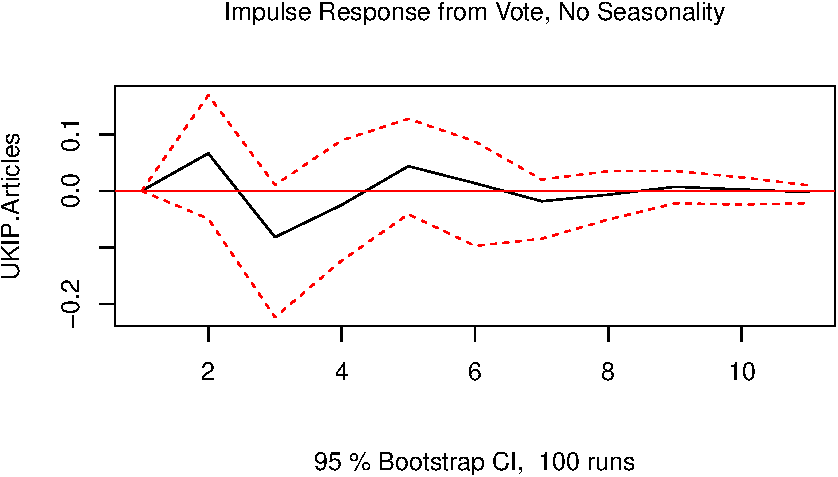
\includegraphics{ukip_media_files/figure-latex/unnamed-chunk-31.pdf}
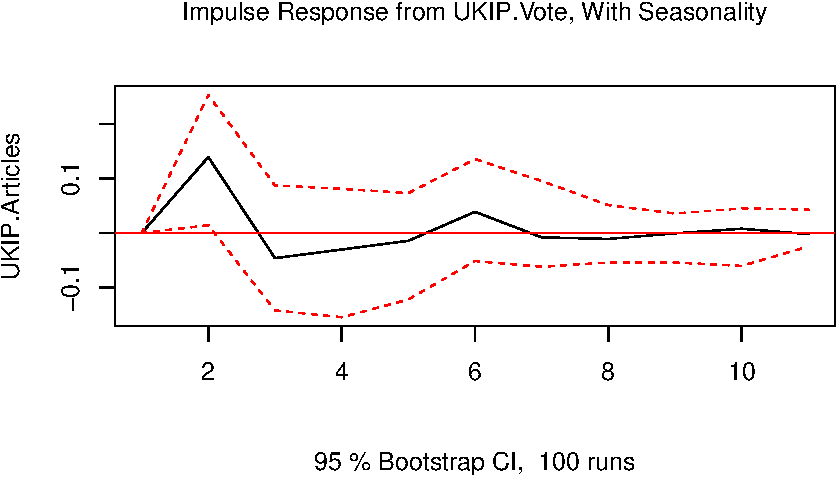
\includegraphics{ukip_media_files/figure-latex/unnamed-chunk-32.pdf}

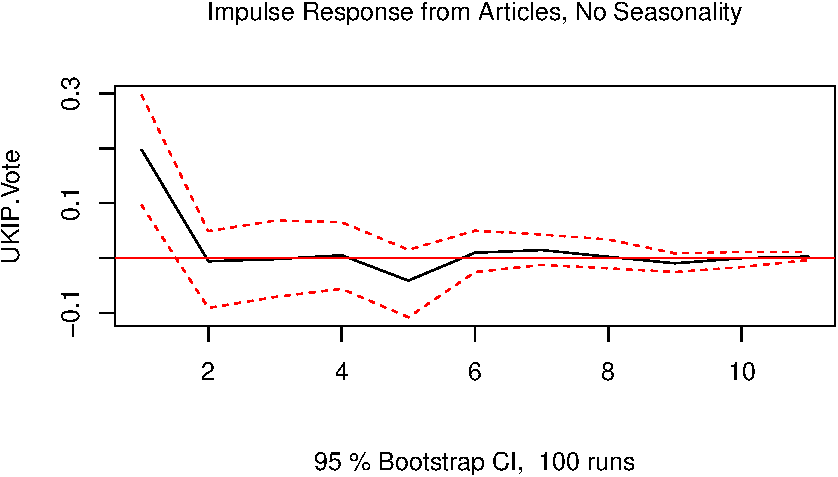
\includegraphics{ukip_media_files/figure-latex/unnamed-chunk-41.pdf}
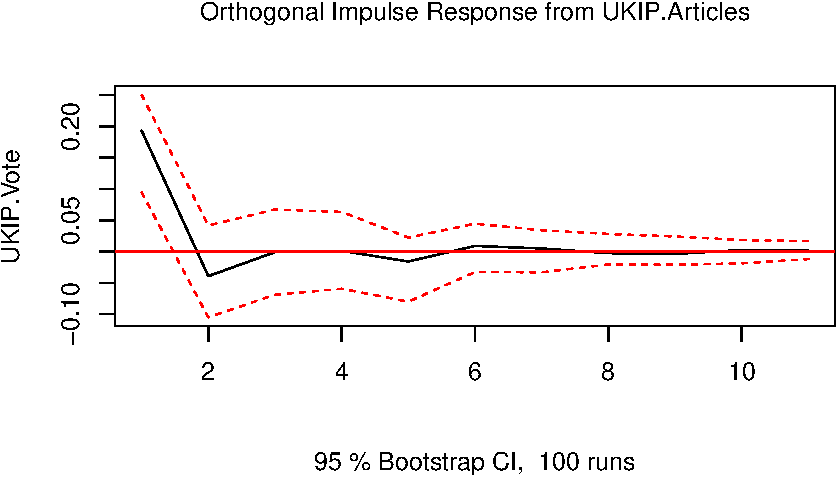
\includegraphics{ukip_media_files/figure-latex/unnamed-chunk-42.pdf}

\subsection{ECM}\label{ecm}

Given the inherent limitations of the VAR approach, the error-correction
model (ECM) is a natural alternative for a hypothesis of positive
feedback. In short, an ECM models changes in a dependent variable as a
function of lagged levels of the dependent variable (reflecting the rate
of error correction or equilibration of the dependent variable) and
changes as well as levels of an independent variable of interest
(short-run and long-run effects, respectively). The ECM is also useful
here because it allows for dependent and independent variables which are
cointegrated. If media coverage and public support each drive each
other, then we should find evidence of this in separate error-correction
models for each variable. The results below show precisely this. Lagged
changes and levels of each variable predict changes in the other
variable with high degrees of statistical significance, suggesting a
change in either variable is associated with an immediate change in the
other variable and a long-run increase in the level of the other
variable. This is precisely what we would expect in a relationship of
positive feedback. All of the models pass the Durbin Watson test for
serial correlation of errors and a t-test of Studentized residuals for
the possibility of outliers. The first model passes the Breusch-Pagan
test for heteroskedasticity; the second model does not pass the
Breusch-Pagan test but the coefficients and standard errors do not
change significantly from those displayed here after using White's
heteroskedasticity-consistent covariance matrix.

\begin{table}[!htbp] \centering 
  \caption{} 
  \label{} 
\begin{tabular}{@{\extracolsep{5pt}}lcc} 
\\[-1.8ex]\hline 
\hline \\[-1.8ex] 
 & \multicolumn{2}{c}{\textit{Dependent variable:}} \\ 
\cline{2-3} 
\\[-1.8ex] & d(UKIP.Articles) & d(UKIP.Vote) \\ 
\\[-1.8ex] & (1) & (2)\\ 
\hline \\[-1.8ex] 
 lag(UKIP.Articles, -1) & $-$0.482$^{***}$ &  \\ 
  & (0.070) &  \\ 
  & & \\ 
 lag(UKIP.Vote, 1, lag = 1) & 0.582$^{***}$ &  \\ 
  & (0.123) &  \\ 
  & & \\ 
 diff(UKIP.Vote, 1, lag = 1) & 0.395$^{***}$ &  \\ 
  & (0.137) &  \\ 
  & & \\ 
 trend(UKIP.Articles) & 0.003 &  \\ 
  & (0.002) &  \\ 
  & & \\ 
 lag(UKIP.Vote, -1) &  & $-$0.395$^{***}$ \\ 
  &  & (0.065) \\ 
  & & \\ 
 lag(UKIP.Articles, 1, lag = 1) &  & 0.163$^{***}$ \\ 
  &  & (0.038) \\ 
  & & \\ 
 diff(UKIP.Articles, 1, lag = 1) &  & 0.105$^{**}$ \\ 
  &  & (0.042) \\ 
  & & \\ 
 trend(UKIP.Vote) &  & 0.002$^{*}$ \\ 
  &  & (0.001) \\ 
  & & \\ 
 Constant & 1.481$^{***}$ & $-$0.517$^{***}$ \\ 
  & (0.235) & (0.130) \\ 
  & & \\ 
\hline \\[-1.8ex] 
Observations & 133 & 133 \\ 
R$^{2}$ & 0.366 & 0.326 \\ 
Adjusted R$^{2}$ & 0.346 & 0.305 \\ 
Residual Std. Error (df = 128) & 0.631 & 0.352 \\ 
F Statistic (df = 4; 128) & 18.500$^{***}$ & 15.510$^{***}$ \\ 
\hline 
\hline \\[-1.8ex] 
\textit{Note:}  & \multicolumn{2}{r}{$^{*}$p$<$0.1; $^{**}$p$<$0.05; $^{***}$p$<$0.01} \\ 
\end{tabular} 
\end{table}

\pagebreak

\begin{verbatim}
## 
## VAR Estimation Results:
## ========================= 
## Endogenous variables: UKIP.Articles, UKIP.Vote 
## Deterministic variables: both 
## Sample size: 131 
## Log Likelihood: -184.541 
## Roots of the characteristic polynomial:
## 0.605 0.605 0.582 0.582 0.479 0.479
## Call:
## VAR(y = diffvars, type = "both", lag.max = 10, ic = "AIC")
## 
## 
## Estimation results for equation UKIP.Articles: 
## ============================================== 
## UKIP.Articles = UKIP.Articles.l1 + UKIP.Vote.l1 + UKIP.Articles.l2 + UKIP.Vote.l2 + UKIP.Articles.l3 + UKIP.Vote.l3 + const + trend 
## 
##                   Estimate Std. Error t value Pr(>|t|)    
## UKIP.Articles.l1 -0.361181   0.096140   -3.76  0.00026 ***
## UKIP.Vote.l1      0.184839   0.172663    1.07  0.28648    
## UKIP.Articles.l2 -0.342776   0.097313   -3.52  0.00060 ***
## UKIP.Vote.l2     -0.086422   0.181688   -0.48  0.63516    
## UKIP.Articles.l3 -0.214449   0.094362   -2.27  0.02478 *  
## UKIP.Vote.l3     -0.112182   0.170214   -0.66  0.51109    
## const             0.044084   0.129619    0.34  0.73436    
## trend             0.000428   0.001645    0.26  0.79539    
## ---
## Signif. codes:  0 '***' 0.001 '**' 0.01 '*' 0.05 '.' 0.1 ' ' 1
## 
## 
## Residual standard error: 0.712 on 123 degrees of freedom
## Multiple R-Squared: 0.184,   Adjusted R-squared: 0.138 
## F-statistic: 3.97 on 7 and 123 DF,  p-value: 0.000605 
## 
## 
## Estimation results for equation UKIP.Vote: 
## ========================================== 
## UKIP.Vote = UKIP.Articles.l1 + UKIP.Vote.l1 + UKIP.Articles.l2 + UKIP.Vote.l2 + UKIP.Articles.l3 + UKIP.Vote.l3 + const + trend 
## 
##                   Estimate Std. Error t value Pr(>|t|)    
## UKIP.Articles.l1  0.105038   0.055237    1.90    0.060 .  
## UKIP.Vote.l1     -0.408589   0.099203   -4.12  6.9e-05 ***
## UKIP.Articles.l2  0.096074   0.055911    1.72    0.088 .  
## UKIP.Vote.l2     -0.251028   0.104388   -2.40    0.018 *  
## UKIP.Articles.l3  0.085342   0.054215    1.57    0.118    
## UKIP.Vote.l3     -0.088077   0.097796   -0.90    0.370    
## const             0.009881   0.074472    0.13    0.895    
## trend             0.000162   0.000945    0.17    0.864    
## ---
## Signif. codes:  0 '***' 0.001 '**' 0.01 '*' 0.05 '.' 0.1 ' ' 1
## 
## 
## Residual standard error: 0.409 on 123 degrees of freedom
## Multiple R-Squared: 0.129,   Adjusted R-squared: 0.079 
## F-statistic: 2.59 on 7 and 123 DF,  p-value: 0.0157 
## 
## 
## 
## Covariance matrix of residuals:
##               UKIP.Articles UKIP.Vote
## UKIP.Articles         0.507     0.140
## UKIP.Vote             0.140     0.167
## 
## Correlation matrix of residuals:
##               UKIP.Articles UKIP.Vote
## UKIP.Articles         1.000     0.482
## UKIP.Vote             0.482     1.000
\end{verbatim}

\begin{verbatim}
## 
## VAR Estimation Results:
## ========================= 
## Endogenous variables: UKIP.Articles, UKIP.Vote 
## Deterministic variables: both 
## Sample size: 131 
## Log Likelihood: -158.491 
## Roots of the characteristic polynomial:
## 0.69 0.69 0.596 0.404 0.404 0.307
## Call:
## VAR(y = diffvars, type = "both", season = 12L, lag.max = 10, 
##     ic = "AIC")
## 
## 
## Estimation results for equation UKIP.Articles: 
## ============================================== 
## UKIP.Articles = UKIP.Articles.l1 + UKIP.Vote.l1 + UKIP.Articles.l2 + UKIP.Vote.l2 + UKIP.Articles.l3 + UKIP.Vote.l3 + const + trend + sd1 + sd2 + sd3 + sd4 + sd5 + sd6 + sd7 + sd8 + sd9 + sd10 + sd11 
## 
##                   Estimate Std. Error t value Pr(>|t|)    
## UKIP.Articles.l1 -0.553388   0.102741   -5.39  4.0e-07 ***
## UKIP.Vote.l1      0.397480   0.172407    2.31    0.023 *  
## UKIP.Articles.l2 -0.448840   0.109289   -4.11  7.7e-05 ***
## UKIP.Vote.l2      0.250204   0.187904    1.33    0.186    
## UKIP.Articles.l3 -0.245201   0.100207   -2.45    0.016 *  
## UKIP.Vote.l3      0.135564   0.173258    0.78    0.436    
## const             0.057340   0.119606    0.48    0.633    
## trend             0.000267   0.001520    0.18    0.861    
## sd1              -0.082795   0.286185   -0.29    0.773    
## sd2               0.260127   0.288265    0.90    0.369    
## sd3               0.526146   0.288290    1.83    0.071 .  
## sd4               0.695356   0.288482    2.41    0.018 *  
## sd5              -0.153701   0.292212   -0.53    0.600    
## sd6              -0.611966   0.293349   -2.09    0.039 *  
## sd7              -0.630215   0.300718   -2.10    0.038 *  
## sd8               0.071458   0.299959    0.24    0.812    
## sd9               0.202142   0.289676    0.70    0.487    
## sd10              0.111573   0.288612    0.39    0.700    
## sd11              0.181855   0.289233    0.63    0.531    
## ---
## Signif. codes:  0 '***' 0.001 '**' 0.01 '*' 0.05 '.' 0.1 ' ' 1
## 
## 
## Residual standard error: 0.655 on 112 degrees of freedom
## Multiple R-Squared: 0.371,   Adjusted R-squared: 0.27 
## F-statistic: 3.67 on 18 and 112 DF,  p-value: 1.1e-05 
## 
## 
## Estimation results for equation UKIP.Vote: 
## ========================================== 
## UKIP.Vote = UKIP.Articles.l1 + UKIP.Vote.l1 + UKIP.Articles.l2 + UKIP.Vote.l2 + UKIP.Articles.l3 + UKIP.Vote.l3 + const + trend + sd1 + sd2 + sd3 + sd4 + sd5 + sd6 + sd7 + sd8 + sd9 + sd10 + sd11 
## 
##                   Estimate Std. Error t value Pr(>|t|)    
## UKIP.Articles.l1  0.059543   0.062763    0.95   0.3448    
## UKIP.Vote.l1     -0.405605   0.105321   -3.85   0.0002 ***
## UKIP.Articles.l2  0.066044   0.066763    0.99   0.3247    
## UKIP.Vote.l2     -0.223278   0.114788   -1.95   0.0543 .  
## UKIP.Articles.l3  0.051490   0.061215    0.84   0.4021    
## UKIP.Vote.l3     -0.086371   0.105841   -0.82   0.4162    
## const             0.004733   0.073066    0.06   0.9485    
## trend             0.000305   0.000929    0.33   0.7434    
## sd1              -0.174712   0.174826   -1.00   0.3198    
## sd2               0.162045   0.176097    0.92   0.3594    
## sd3               0.168527   0.176112    0.96   0.3407    
## sd4               0.329795   0.176230    1.87   0.0639 .  
## sd5               0.258714   0.178508    1.45   0.1500    
## sd6              -0.000607   0.179202    0.00   0.9973    
## sd7              -0.009899   0.183704   -0.05   0.9571    
## sd8               0.043452   0.183241    0.24   0.8130    
## sd9               0.010503   0.176959    0.06   0.9528    
## sd10             -0.149452   0.176309   -0.85   0.3984    
## sd11              0.157363   0.176688    0.89   0.3750    
## ---
## Signif. codes:  0 '***' 0.001 '**' 0.01 '*' 0.05 '.' 0.1 ' ' 1
## 
## 
## Residual standard error: 0.4 on 112 degrees of freedom
## Multiple R-Squared: 0.24,    Adjusted R-squared: 0.118 
## F-statistic: 1.97 on 18 and 112 DF,  p-value: 0.0171 
## 
## 
## 
## Covariance matrix of residuals:
##               UKIP.Articles UKIP.Vote
## UKIP.Articles         0.429     0.127
## UKIP.Vote             0.127     0.160
## 
## Correlation matrix of residuals:
##               UKIP.Articles UKIP.Vote
## UKIP.Articles         1.000     0.483
## UKIP.Vote             0.483     1.000
\end{verbatim}

\begin{figure}[htbp]
\centering
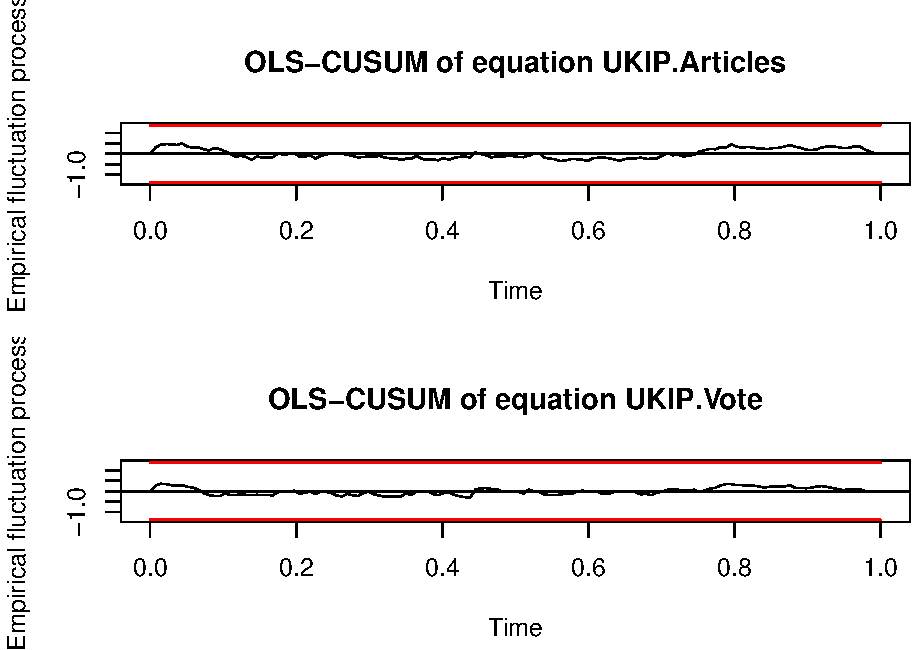
\includegraphics{ukip_media_files/figure-latex/supplementary.pdf}
\caption{plot of chunk supplementary}
\end{figure}

\pagebreak

\section*{References}\label{references}
\addcontentsline{toc}{section}{References}

Boomgaarden, Hajo G, and Rens Vliegenthart. 2007. ``Explaining the Rise
of Anti-Immigrant Parties: The Role of News Media Content.''
\emph{Electoral Studies} 26 (2): 404--17.

---------. 2009. ``How News Content Influences Anti-Immigration
Attitudes: Germany, 19932005.'' \emph{European Journal of Political
Research} 48 (4): 516--42.

Bos, Linda, Wouter van der Brug, and Claes de Vreese. 2011. ``How the
Media Shape Perceptions of Right-Wing Populist Leaders.''
\emph{Political Communication} 28 (2): 182--206.

Goodwin, Matthew, and Robert Ford. 2013. ``Just How Much Media Coverage
Does UKIP Get?''
\url{http://www.newstatesman.com/politics/2013/11/just-how-much-media-coverage-does-ukip-get}.

Ipsos-MORI. ``Voting Intention in Great Britain: Recent Trends.''
\url{https://www.ipsos-mori.com/researchpublications/researcharchive/poll.aspx?oItemId=107\&view=wide}.

``Nexis.''

Soussi, Alasdair. 2014. ``Did British Media Help the UKIP Win EU Poll?''
\url{http://www.aljazeera.com/indepth/features/2014/06/did-british-media-help-ukip-win-eu-poll-20146313346918679.html}.

Stevenson, Alex. 2014. ``Caroline Lucas Points Finger at Media's Farage
Obsession.''
\url{http://www.politics.co.uk/news/2014/05/29/ukip-victory-caroline-lucas-points-finger-at-media-s-farage}.

Sweeney, Mark. 2015. ``BBC Prepares to Boost Ukip Coverage as It Ranks
It a Larger Party in Election.''
\url{http://www.theguardian.com/media/2015/jan/15/bbc-prepares-to-boost-ukip-coverage-as-it-ranks-it-a-larger-party-in-election}.

Syal, Rajeev. 2015. ``Ukip Faces Crisis After Suspensions and Racism
Claims.''
\url{http://www.theguardian.com/politics/2015/mar/20/ukip-faces-crisis-two-parliamentary-candidates-suspended-one-resigns}.

Vliegenthart, Rens. 2014. ``Moving up. Applying Aggregate Level Time
Series Analysis in the Study of Media Coverage.'' \emph{Quality \&
Quantity} 48 (5): 2427--45.

Webb, Robert. 2014. ``Ukip Trades in the Language of Fear and Division.
The Left Must Not Humour Its Anti-Politics Crusade.''
\url{http://www.newstatesman.com/politics/2014/05/ukip-trades-language-fear-and-division-left-must-not-humour-its-anti-politics}.

Wintour, Patrick. 2015. ``Ofcom Deals Blow to Greens Election Debate
Hopes but Boosts Ukips.''
\url{http://www.theguardian.com/politics/2015/jan/08/ofcom-blow-green-party-election-debate-boost-ukips}.

\end{document}
